\centering
\begin{figure}[h!]
  \vspace{-30mm}
  \begin{subfigure}{0.5\textwidth}
    \includegraphics[height=60mm]{n_500_n3_3d_v2}
    \caption{$n^{3}$ timescale}
    \label{fig:100s3}
  \end{subfigure}%
  \begin{subfigure}{0.5\textwidth}
    \includegraphics[height=60mm]{n_500_2n3_3d_v2}
    \caption{$n^{2}$ timescale}
    \label{fig:100s3}
  \end{subfigure}%
  \caption{Evolution of degrees. ($n=500$, $m=250000$)}
  \label{fig:n500_3d}
\end{figure}

\begin{figure}[h!]
  \vspace{-5mm}
  \centering
  \begin{subfigure}{0.5\textwidth}
    \centering
    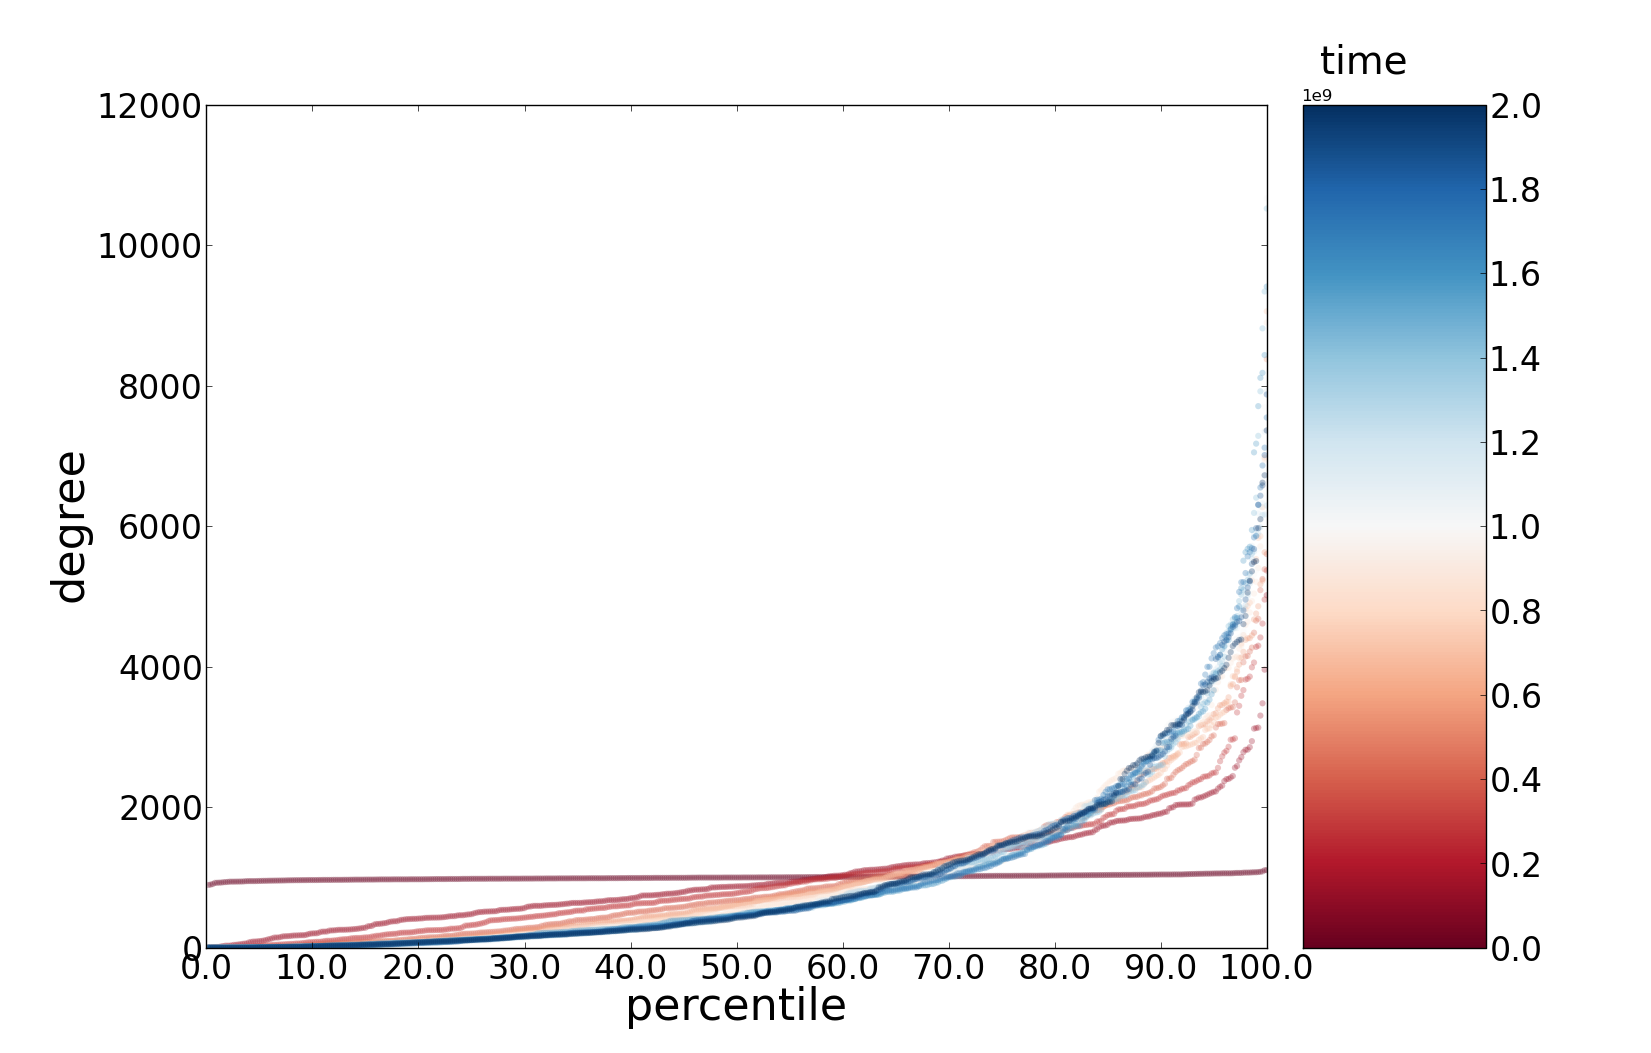
\includegraphics[height=50mm]{n_500_n3_deg_percentile}
    \caption{$n^{3}$ timescale}
    \label{fig:100s3}
  \end{subfigure}%
  \begin{subfigure}{0.5\textwidth}
    \centering
    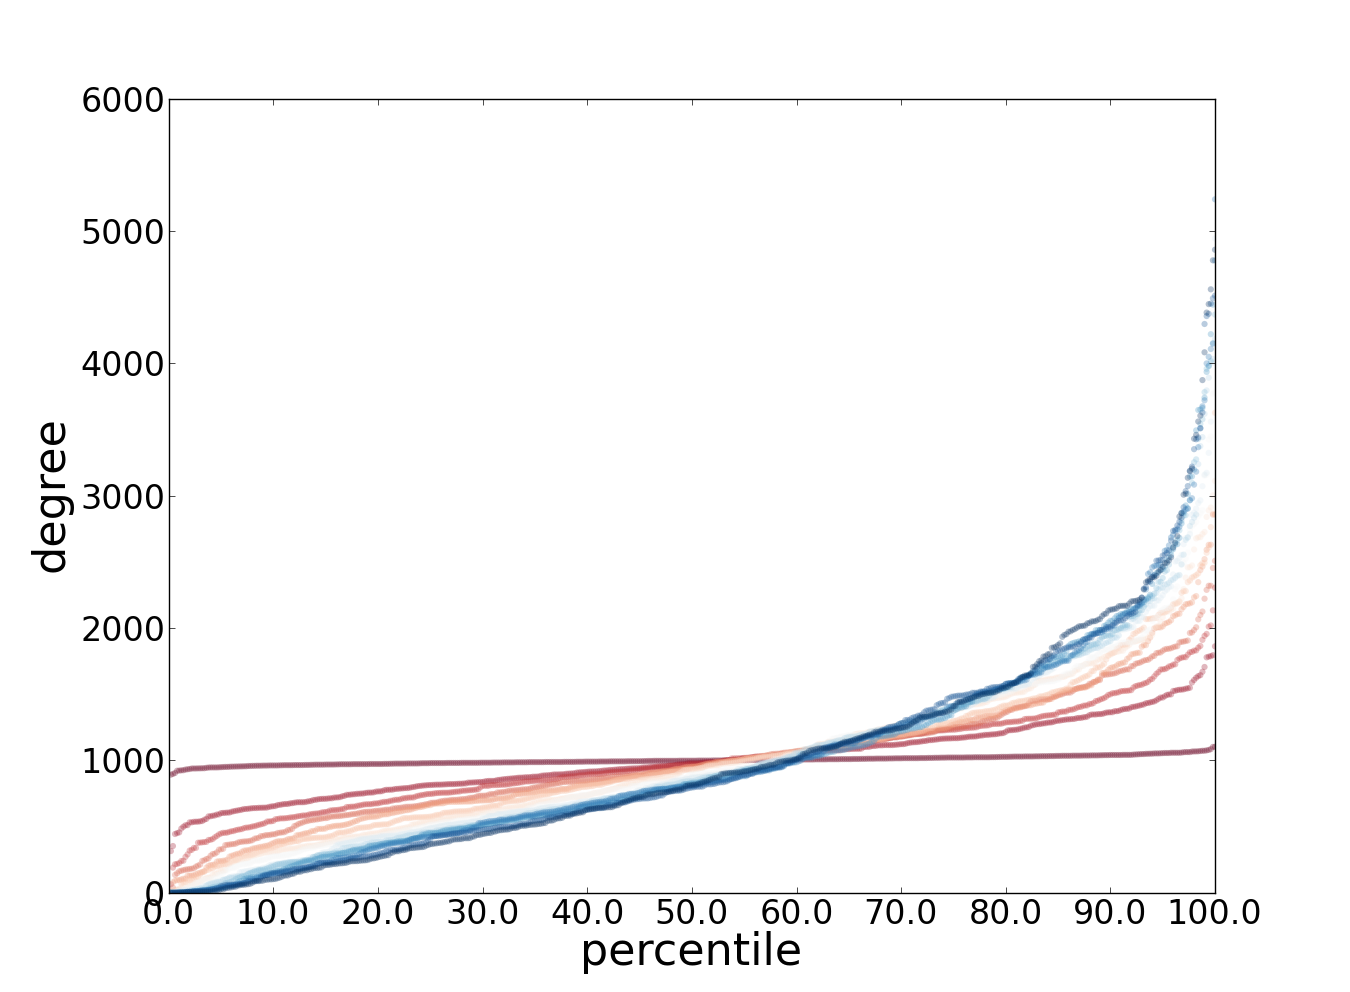
\includegraphics[height=50mm]{n_500_2n3_deg_percentile}
    \caption{$n^{2}$ timescale}
    \label{fig:100s3}
  \end{subfigure}%
  \caption{Evolution of degrees and percentiles, a projection of Fig. \ref{fig:n500_3d} along the time axis. ($n=500$, $m=250000$)}
\end{figure}

\begin{figure}[h!]
  \vspace{-5mm}
  \centering
  \begin{subfigure}{0.5\textwidth}
    \centering
    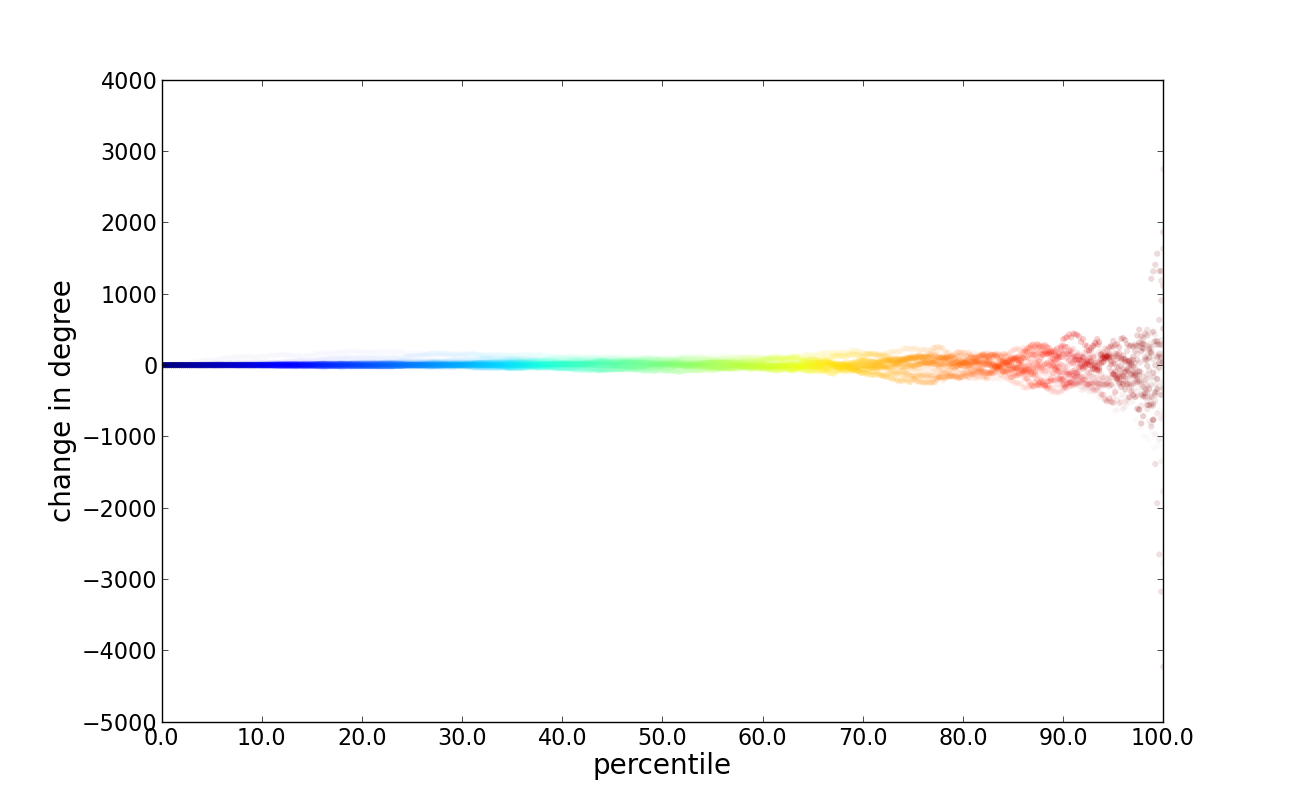
\includegraphics[height=60mm]{n_500_n3_degchange_percentile}
    \caption{$n^{3}$ timescale}
    \label{fig:100s3}
  \end{subfigure}%
  \begin{subfigure}{0.5\textwidth}
    \centering
    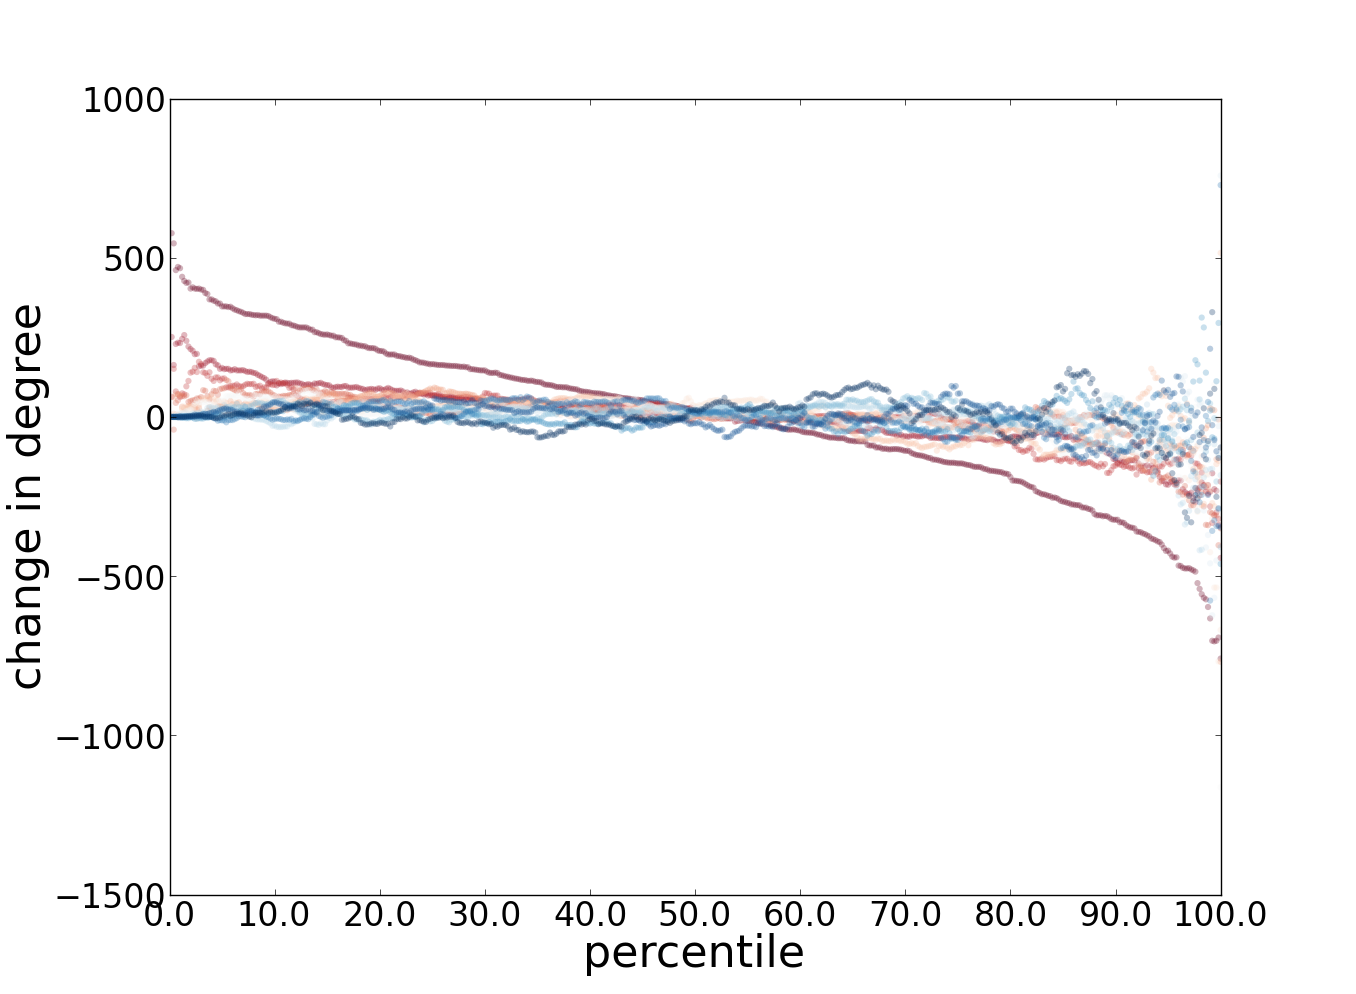
\includegraphics[height=60mm]{n_500_2n3_degchange_percentile}
    \caption{$n^{2}$ timescale}
    \label{fig:100s3}
  \end{subfigure}%
  \caption{Change in degree distribution between each step plotted against percentiles. ($n=500$, $m=250000$)}
\end{figure}

\begin{figure}[h!]
  \vspace{-5mm}
  \begin{subfigure}{0.5\textwidth}
    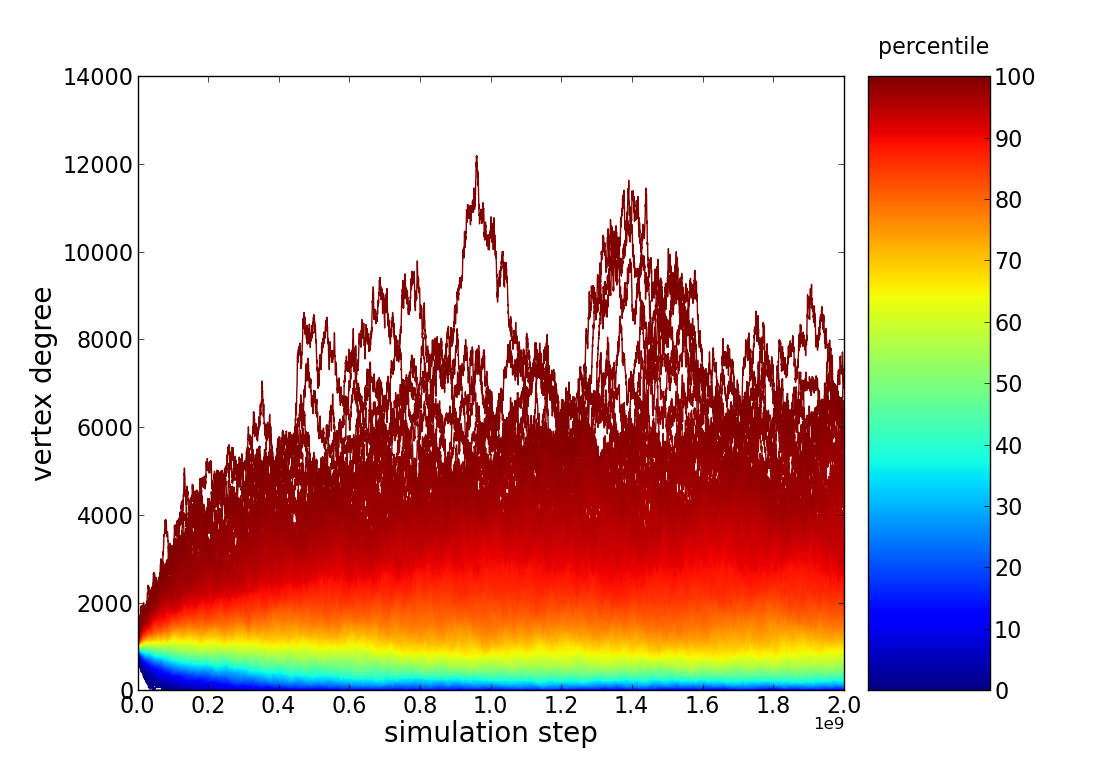
\includegraphics[height=50mm]{n_500_n3_deg_step}
    \caption{$n^{3}$ timescale}
    \label{fig:100s3}
  \end{subfigure}%
  \begin{subfigure}{0.5\textwidth}
    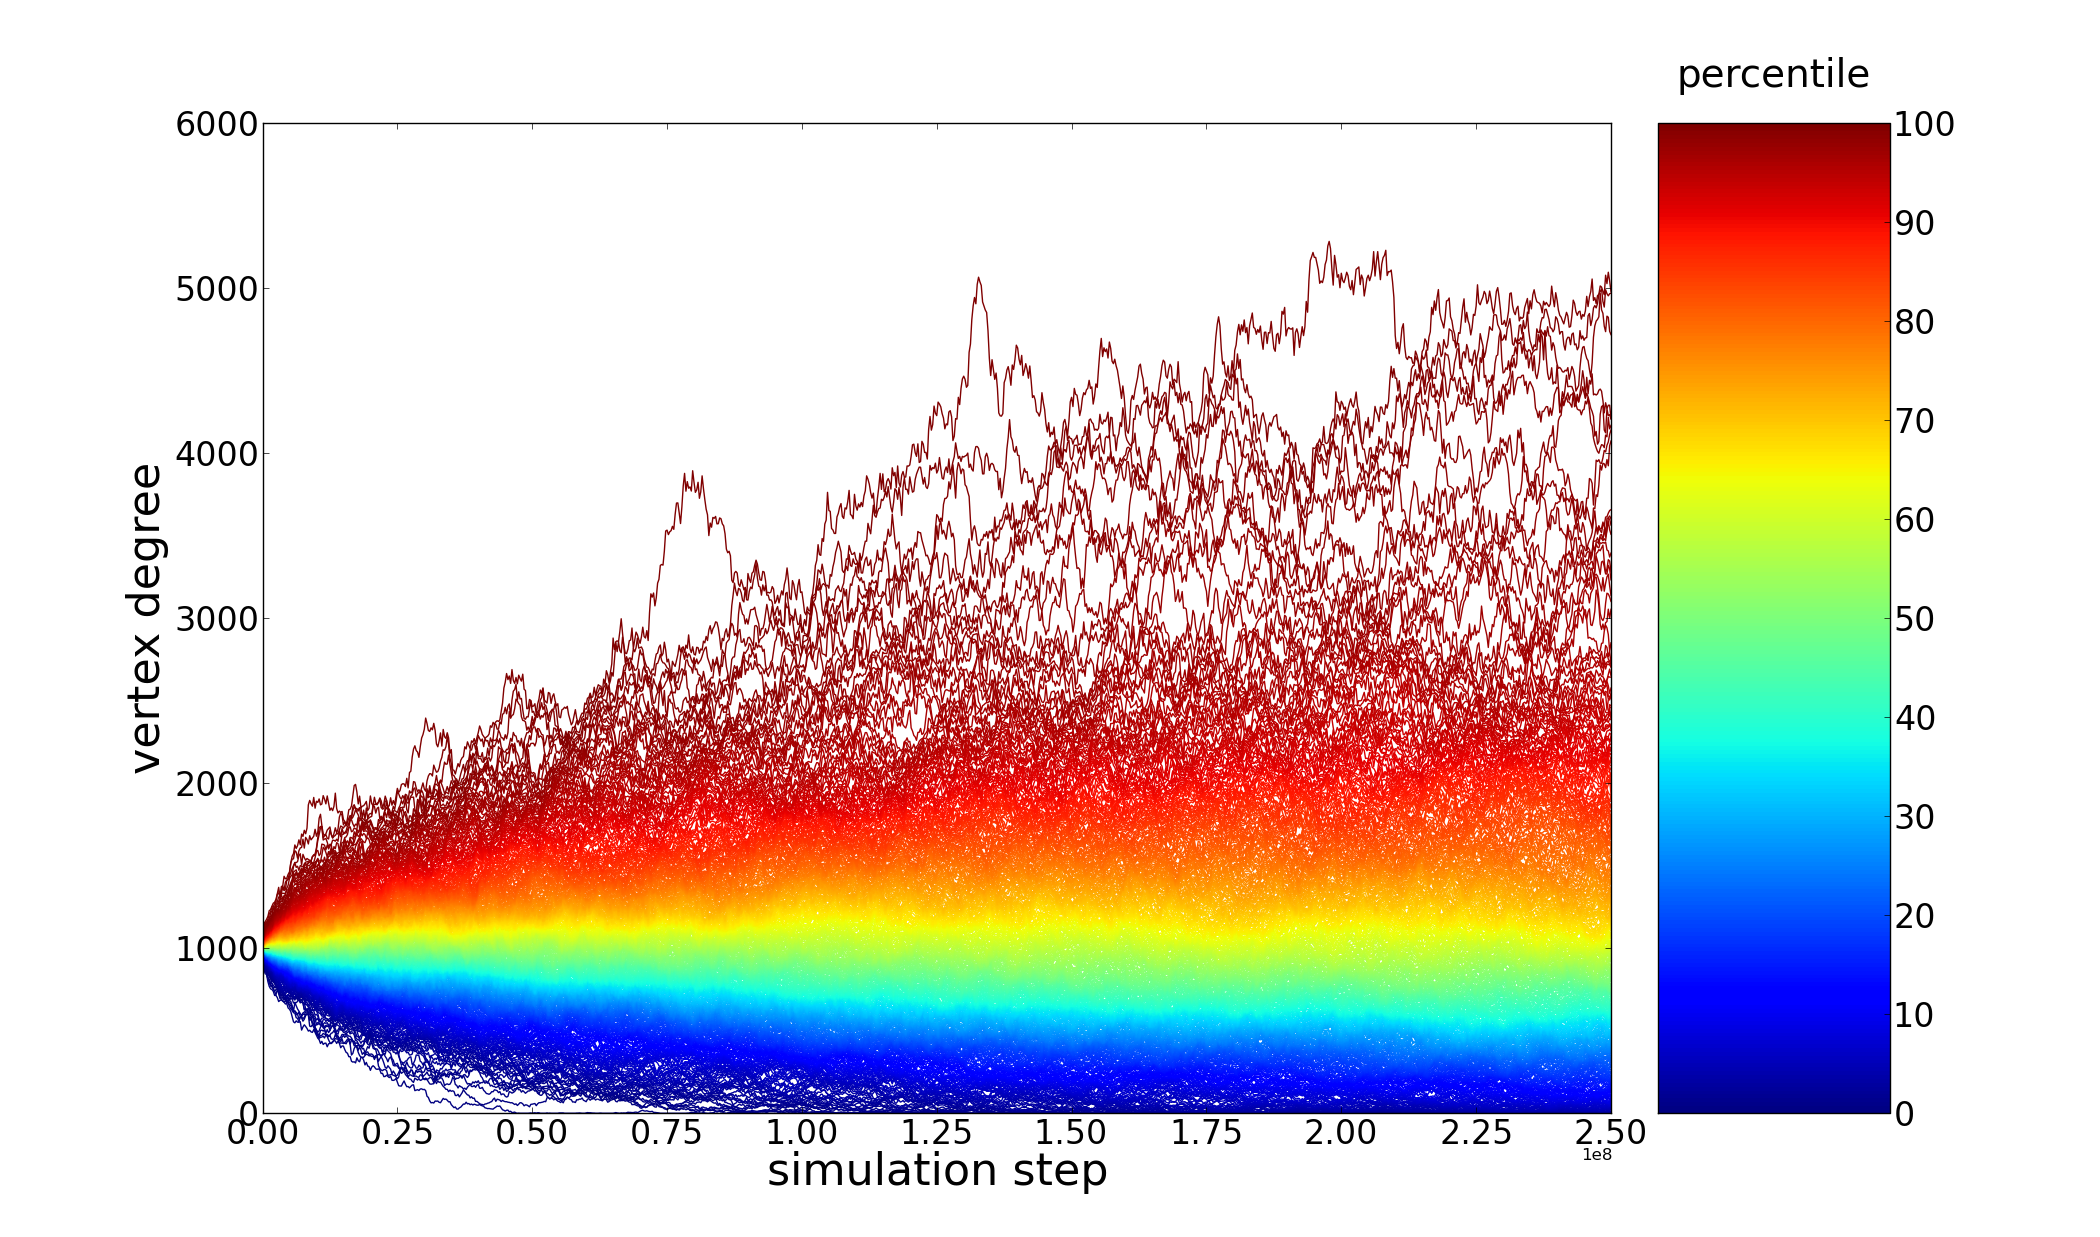
\includegraphics[height=50mm]{n_500_2n3_deg_step}
    \caption{$n^{2}$ timescale}
    \label{fig:100s3}
  \end{subfigure}%
  \caption{Evolution of degree distribution. Color indicates percentile, i.e. the median degree at each step is colored green. ($n=500$, $m=250000$)}
\end{figure}

%% \begin{figure}[h!]
%%   \centering
%%   \includegraphics[height=60mm]{n_500_short}
%%   \caption{$n^{2}$ timescale, $n=500$, $m=250000$}
%%   \label{fig:500sv}
%% \end{figure}
%% \begin{figure}[h!]
%%   \centering
%%   \includegraphics[height=60mm]{n_500_long_3d}
%%   \caption{$n^{3}$ timescale, $n=500$, $m=250000$}
%%   \label{fig:500l3}
%% \end{figure}
%% \begin{figure}[h!]
%%   \centering
%%   \includegraphics[height=60mm]{n_500_long_time}
%%   \caption{$n^{3}$ timescale, $n=500$, $m=250000$}
%%   \label{fig:500lt}
%% \end{figure}
%% \begin{figure}[h!]
%%   \centering
%%   \includegraphics[height=60mm]{n_500_long}
%%   \caption{$n^{3}$ timescale, $n=500$, $m=250000$}
%%   \label{fig:500lv}
%% \end{figure}

%% \begin{figure}[h!]
%%   \centering
%%   \includegraphics[height=60mm]{n_1000_short_3d}
%%   \caption{$n^{2}$ timescale, $n=1000$, $m=1000000$}
%%   \label{fig:1000s3}
%% \end{figure}
%% \begin{figure}[h!]
%%   \centering
%%   \includegraphics[height=60mm]{n_1000_short_time}
%%   \caption{$n^{2}$ timescale, $n=1000$, $m=1000000$}
%%   \label{fig:1000st}
%% \end{figure}
%% \begin{figure}[h!]
%%   \centering
%%   \includegraphics[height=60mm]{n_1000_short}
%%   \caption{$n^{2}$ timescale, $n=1000$, $m=1000000$}
%%   \label{fig:1000sv}
%% \end{figure}
%% \begin{figure}[h!]
%%   \centering
%%   \includegraphics[height=60mm]{n_1000_long_3d}
%%   \caption{$n^{3}$ timescale, $n=1000$, $m=1000000$}
%%   \label{fig:1000l3}
%% \end{figure}
%% \begin{figure}[h!]
%%   \centering
%%   \includegraphics[height=60mm]{n_1000_long_time}
%%   \caption{$n^{3}$ timescale, $n=1000$, $m=1000000$}
%%   \label{fig:1000lt}
%% \end{figure}
%% \begin{figure}[h!]
%%   \centering
%%   \includegraphics[height=60mm]{n_1000_long}
%%   \caption{$n^{3}$ timescale, $n=1000$, $m=1000000$}
%%   \label{fig:1000lv}
%% \end{figure}
